\chptr{Termodimaica - Parte I}
\marginpar{\minitoc}

\section{Introduzione}
In questo capitolo il ruolo dell'energia diventa ancora più
importante. In precedenza abbiamo dimostrato che la differenza di
energia meccanica di un sistema corrisponde al lavoro totale delle
forze non conservative che agiscono sul sistema, quindi $W^\text{NC} = \Delta E$.
In altri termini, l'energia che un sistema possiede viene persa o
acquistata nel caso in cui vi siano forze non conservative che
compiono lavoro su di esso. Ma quindi l'unico modo di ``parlare'',
trasferire energia, ad un sistema dell'universo è quello di compiere
lavoro? In realtà no, come mostreremo parlando di \textit{calore},
un'altra forma di energia \textit{in movimento} come il lavoro, ma
in un certo senso più disordinata.

Ci occuperemo inoltre di sistemi fisici contenenti un numero di
costituenti dell'ordine del numero di Avogadro

\[ N_A = 6 \cdot 10^{23} \]

\noindent Il sistema di questo tipo che più ci interessa è quello
dei gas. Supporremo che i gas sono costituiti da particelle
infinitesime che devono seguire certi comportamenti ideali. Ma
trattandosi di punti materiali, non possiamo studiare questi
sistemi in termini meccanici, secondo la dinamica newtoniana,
come abbiamo sempre fatto? Se seguissimo questa strada, potremmo
non vivere abbastanza per vedere i risultati: Dovremmo prima di
tutto osservare e misurare le caratteristiche cinematiche e
meccaniche di ogni singola particella, quanto meno ad un preciso istante di
tempo (dovremmo dunque misurare tutte le particelle pressoché
contemporaneamente), stilare poi un sistema di equazioni che
descriva le quantità di moto, le energie in gioco ed eventualmente
altre informazioni per analizzare gli urti e prevedere lo stato
futuro del sistema. Due vie alternative sono possibili: La prima è
quella di introdurre nuove grandezze che misurino lo stato globale
del sistema, rinunciando ad elencarne minuziosamente i dettagli come
abbiamo descritto sopra; la seconda, una sorta di compromesso,
è di ricorrere alla statistica. Noi tratteremo qui la prima modalità
per ragioni storiche e semplicità (la seconda, chiamata \textit{meccanica statistica},
è una delle ultime evoluzioni della termodinamica, assai più
complessa della formulazione classica).

In effetti, la ricerca delle relazioni tra le varie proprietà
dei materiali, senza conoscere la loro struttura interna, è l'oggetto
di studio della termodinamica\footnote{Feynman, 44-1}. In realtà cercheremo una spiegazione di certi fenomeni
analizzando ciò che accade nel microscopico, come mostreremo con la
teoria cinetica, ma ciò che soprenderà di più sarà il fatto che effetti
come pressione e variazioni di temperatura sono pressoché indipendenti
dai dettagli interni delle particelle del materiale come le loro singole
collisioni.

\subsection{Sistemi termodinamici}
Le nostre trattazioni avranno per oggetto i \textit{sistemi termodinamici}, per
definizione immersi in un \textit{ambiente esterno}. Ambiente esterno e il suo
contenuto costituiscono l'\textit{universo}, un sistema che per definizione non
è contenuto in un altro ambiente esterno.
Altro oggetto di nostro interesse per lo studio di questi sistemi sono le
\textit{trasformazioni termodinamiche}, ovvero processi nei quali avvengono
scambi di energia e che si osservano nei sistemi elencati sopra. Qualsiasi
cosa può essere un sistema termodinamico, ma l'esempio più classico è quello
della pentola sul fuoco (figura \ref{pentola}), dove il contenuto è il sistema termodinamico mentre
la cucina e il fornello sono l'ambiente esterno. Nel complesso, questi
elementi costituiscono un universo (dunque non necessariamente la
realtà intera o il cosmo!), all'interno del quale avvengono scambi di
energia. Si suppone che questi scambi siano indipendenti da ciò che, se esiste,
si trova fuori dall'universo.

\begin{marginfigure}
    \centering
    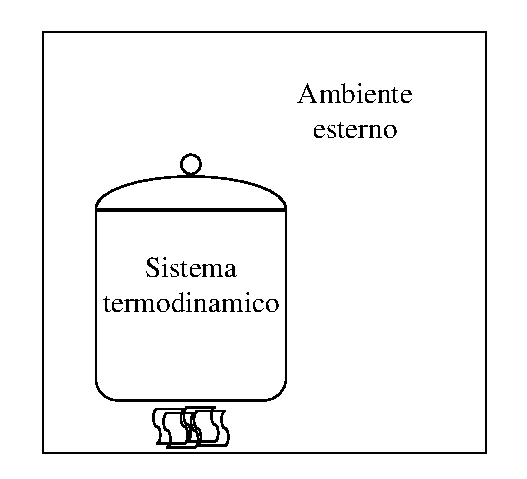
\includegraphics[width = \marginparwidth]{universo_termodinamico.pdf}
    \caption{Un esempio di universo, composto da un sistema termodinamico
    (la pentola) e un ambiente esterno (la stanza). Viene anche mostrato uno
    scambio di energia, mediato dal fuoco.}
    \label{pentola}
\end{marginfigure}


Possiamo classificare i sistemi termodinamici sulla base di due criteri: capacità
di scambiare materia e capacità di scambiare energia con l'ambiente esterno.

\begin{center}
    \begin{tabular}{c | c | c}
        Sistema & Scambia materia & Scambia energia \\
        \hline
        \hline
        \textit{Aperto} & $\surd$ & $\surd$ \\
        \hline
        \textit{Chiuso} & $\times$ & $\surd$ \\
        \hline
        \textit{Isolato} & $\times$ & $\times$
    \end{tabular}
\end{center}

\noindent È immediato chiedersi se esistono sistemi opposti a quelli chiusi, che
scambiano materia ma non energia con l'ambiente esterno. Ma questo
è impossibile, perché vale
\begin{align}
    E = mc^2
\end{align}
\noindent dove $c$ corrisponde alla velocità della luce nel vuoto.
Questa celebre equazione, anche se più complessa di quel che
sembra, mostra che ogni corpo possiede una certa energia $E$ per il semplice
motivo che esso possiede una massa $m$.

\subsection{Variabili termodinamiche}
Le \textit{variabili} (o \textit{coordinate}) \textit{termodinamiche}
sono gli strumenti che in termodinamica sostituiscono le proprietà
cinematiche a cui eravamo abituati in meccanica: lo spazio e il tempo,
che ci permettevano di descrivere il moto dei punti materiali.
Come già discusso precedentemente, questa sostituzione ha motivi pratici.
Le variabili termodinamiche fondamentali sono \textit{pressione} $p$
(rapporto tra il modulo di una forza perpendicolare ad una superficie
e l'area della superficie stessa), \textit{temperatura} $T$ (espressione
quantitativa della nostra sensazione di caldo e freddo), \textit{volume} $V$
e massa $m$\footnote{In termodinamica è spesso presente un'influenza da parte
della chimica, quindi alla massa si preferisce la \textit{mole} (come
la massa, si riferisce a quantità di materia).}. Come poi in cinematica
utilizzavamo un sistema di assi cartesiani, anche ora utilizziamo lo
stesso strumento matematico (il piano $pV$, pressione-volume) accoppiandolo però con le coordinate termodinamiche
appena introdotte. Il piano $pV$ sarà costituito da un solo quadrante,
perché sia il volume che la pressione possono assumere valori non
negativi\footnote{Anzi positivi, come accade spesso nella realtà.}.

Le variabili termodinamiche si suddividono in due categorie:
grandezze \textit{intensive} ed \textit{estensive}. Il valore delle
grandezze intensive non dipende dalla quantità di materia o dall'estensione
del campione esaminato, ma soltanto dalla sua natura e/o dalle
condizioni in cui si trova e possono essere misurate localmente.
La temperatura di una stanza, per esempio, non dipende dalle sue
dimensioni o dal tipo di aria che esso contiene. Dall'altro lato,
le estensive dipendono dalla quantità di materia esaminata e dalla
sua estensione.

\begin{center}
    \begin{tabular}{c || c}
        Grandezze intensive & Grandezze estensive\\
        \hline
        $p$, $T$ & $V$, $m$
    \end{tabular}
\end{center}


\subsection{Trasformazioni termodinamiche ed equilibrio}
I sistemi termodinamici possono essere descritti dalle coordinate
termodinamiche appena introdotte, che giacciono su un piano. Un
sistema che viene idealmente rappresentato da un punto fisso sul
piano $pV$ è in uno \textit{stato di equilibrio termodinamico},
nel quale le condizioni di pressione, volume e temperatura rimangono
costanti col passare del tempo.
Un sistema si dice in equilibrio termodinamico se esso rispetta i seguenti equilibri:
\begin{enumerate}
    \item \textit{Equilibrio meccanico}: lo stato non è sottoposto a forze totali non nulle,
    in qualsiasi coppia delle sue parti.

    \item \textit{Equilibrio chimico}: non esiste alcuna reazione chimica tra una qualsiasi
    coppia di parti del sistema.

    \item \textit{Equilibrio termico}: per ogni coppia di parti, la temperatura è la stessa.
\end{enumerate}

\noindent Per ``parti'' di un sistema intendiamo sottoinsiemi
abbastanza piccoli rispetto al sistema originale ma allo stesso
tempo sufficientemente grandi affiché gli strumenti della termodinamica
funzionino.


Un sistema può ovviamente muoversi all'interno del piano $pV$, cambiando
i propri parametri termodinamici e spostandosi tra due stati differenti.
Questi movimenti sono chiamati \textit{trasformazioni termodinamiche} e
vedremo più avanti che sono processi che coinvolgono scambi di energia
tra sistema termodinamico e ambiente esterno. Nel mondo reale, approssimare
sperimentalmente la curva di una trasformazione sul piano $pV$ è
estremamente difficile e dunque, se un sistema passa dallo stato $A$
ad uno differente $B$, non vi è garanzia di equilibrio nel percorso
tra i due punti. Per ora, ciò ci permette solo di ``accontentarci'' di
stimare teoricamente l'energia scambiata e i parametri in una trasformazione
termodinamica. Per questo motivo, sottointenderemo la seguente assunzione
in questo capitolo: tutte le trasformazioni trattate sono \textit{quasistatiche}\footnote{Da non confondere con le trasformazioni \textit{reversibili}, trattate più avanti.}
(a meno che non venga specificato diversamente).

\begin{tcolorbox}[colback = yellow!30, colframe = yellow!30!black, title = {Trasformazione quasistatica}]
    Trasformazione termodinamica ideale nella quale il sistema termodinamico
    attraversa equilibri successivi. Data una trasformazione $\tau$ quasistatica
    sul piano $pV$, tutti i punti di $\tau$ sono stati di equilibrio.
\end{tcolorbox}

\noindent Le trasformazioni quasistatiche sono irriproducibili sperimentalmente,
perché, affinché ad \textit{ogni} istante il sistema si trovi in uno stato
di equilibrio, è necessario variare le sue coordinate termodinamiche in
quantità infinitesime e in tempi sufficienetemente lunghi in modo da non
rompere gli equilibri.



\subsection{Quantificare caldo e freddo}
Abbiamo tutti un'idea intuitiva della temperatura, della quale facciamo
esperienza col tatto. Non tutti però percepiscono caldo e freddo allo
stesso modo e spesso non siamo bravi a stimare con precisione la
temperatura di un oggetto\footnote{\href{https://www.youtube.com/watch?v=vqDbMEdLiCs}{\textcolor{blue}{Misconception about Temperature - Veritasium}}.}.
Nella storia passata siamo riusciti ad individuare alcuni metodi in
grado di misurare indirettamente la temperatura, grazie agli effetti
della sua variazione. Il più comune di questi è la dilatazione dei
metalli. I vecchi e classici termometri a mercurio sfruttano questo
principio.

\begin{tcolorbox}[colback = yellow!30, colframe = yellow!30!black, title = {Termometro}]
Strumento che, data la variazione di una certa grandezza $X$ per
via di variazioni di temperatura, permette di misurare quest'ultima.
\end{tcolorbox}

...discorso su calibrazione ecc...

Se la misura che i termometri ci forniscono è indiretta, come possiamo
essere sicuri che il valore che otteniamo sia quello corretto? Il
principio zero, di cui si parla nella prossima sezione, ci consente di fidarci dei termometri.


\section{Principio zero}
\begin{tcolorbox}[colback = red!30, colframe = red!30!black, title = {Primo zero della termodinamica}]
Se un corpo $A$ è in equilibrio termico con $B$ e $B$ lo è con un terzo
corpo $C$, allora $A$ è in equilibrio termico con $C$.

In particolare, se $T_A = T_B$ e $T_B = T_C$, allora $T_A = T_C$; cioè
i corpi possiedono la medesima temperatura.
\end{tcolorbox}

\noindent Sottolineamo che le equivalenze espresse dal principio non
sono dedotte da proprietà logico-matematiche, ma sono affermazioni
forndate puramente su evidenze sperimentali.

Alcuni testi espongono il principio zero anticipando un fatto dell'universo
che noi affrontiamo nella seconda parte, cioè che due corpi, uno caldo e
uno freddo, in contatto termico tra loro raggiungeranno la stessa temperatura,
se si attende un tempo sufficientemente lungo. Precisiamo che l'equilibrio
termico, nel mondo reale, è un equilibrio dinamico. Ciò significa che
la temperatura di due corpi in contatto termico non è sempre esattamente la
stessa, ma può subire microscopiche fluttuazioni che tuttavia si possono
spesso trascurare.


\section{Esperienza di Joule}
A metà del Diciannovesimo secolo, James Prescott Joule compì alcuni
esperimenti celebri che misero in luce il legame tra alcune forme di
energia e temperatura. Il più noto esperimento è quello del mulinello,
con il quale Joule mostrò \textit{l'equivalente meccanico del calore}.
Il dispositivo di Joule consisteva in un serbatoio adiabatico contenente
acqua, la cui temperatura veniva controllata per mezzo di un termometro
infilato in un'apertura del serbatoio. Nell'acqua vi era poi immerso
un mulinello azionato dall'esterno da un sistema di carrucole e masse
in caduta libera. L'esperimento consisteva nel sollevare una certa
massa totale $m$ ad una altezza $h$; cadendo, la massa avrebbe messo
il mulinello in rotazione, agitando l'acqua del serbatoio. Joule
osservò che la temperatura dell'acqua aumentava dopo la caduta della
massa e l'incremento di temperatura era proporzionale alla massa e all'altezza.

Un'analisi energetica del sistema mette in luce che un certo lavoro è
stato compiuto sull'acqua del serbatoio:

\[ W = mgh \]

\noindent Per principio di conservazione dell'energia, il lavoro non
può essere sparito nel nulla. L'effetto della caduta della massa è stato però un aumento di temperatura.
La conclusione più ragionevole è che temperatura ed energia sono tra
loro legati da qualche relazione.




\section{Principio primo}
Con il primo principio della termodinamica introduciamo una semplice
legge che descrive le modalità con le quali i sistemi dell'universo
comunicano tra loro, cioè come essi scambiano energia. Non a caso
esponiamo dettagliatamente in questa sezione i tre meccanismi
principali con i quali il calore si ``muove'' (conduzione, convezione,
irraggiamento).


\subsection{Lavoro ed energia interna}
Come abbiamo osservato con Joule, è sperimentalmente evidente che
se si compie lavoro sull'acqua, essa
aumenta la propria temperatura. Inoltre, se la temperatura iniziale
dell'acqua è la stessa in tutti gli esperimenti e il lavoro compiuto
è sempre uguale, allora la temperatura finale sarà anch'essa la stessa
in tutte le situazioni. Da ciò si può dedurre che l'aumento di
temperatura non dipende dalla natura del lavoro. Cos'è allora la
temperatura? Non possiamo ancora rispondere a questa domanda, ma
sicuramente sappiamo che essa è legata in qualche modo all'energia,
quantomeno al lavoro.

La temperatura ci fornisce un'informazione sullo stato di
un corpo, cioè una proprietà che lo caratterizza in un dato istante,
in una certa situazione. Il lavoro è invece qualcosa di dinamico,
una ``energia in movimento'' dovuta al moto di qualche cosa. Il
lavoro si trasferisce da corpo a corpo e ne altera una proprietà di
stato, il cui indicatore è la temperatura. L'energia del lavoro,
allora, si può immagazzinare nei corpi, come abbiamo visto parlando
di (variazione di) energia potenziale $\Delta\mathcal{U} = -W$.
Anche qui potremmo parlare di una qualche energia potenziale, ma
non possiamo denominarla in questo modo perché in generale non
si osservano forze conservative in azione. Introduciamo allora
l'energia interna di un sistema, che, come si è osservato
dagli esperimenti, è esprimibile come funzione della temperatura

\[ U = U(T) \]

\noindent Non possiamo ancora dire con precisione quale sia
la formula chiusa che unisce le due quantità, ma sicuramente
gli esperimenti confermano che energia interna e temperatura
sono legate da una qualche costante di proporzionalità:

\[ U \propto T \]

\subsection{Calore}
Dal paragrafo precedente abbiamo scoperto che si può dedurre il
contenuto energetico di un sistema in funzione della sua temperatura.
Con Joule, però, abbiamo visto che, per aumentare la temperatura di
un sistema, è necessario compiere del lavoro su di esso. Ma per
esperienza sappiamo che un corpo freddo può essere riscaldato da uno
più caldo. In una situazione del genere, tuttavia, non si osserva alcun lavoro in azione. Per
spiegare questo fenomeno, la fisica ha introdotto una quantità
energetica nuova: il calore.

\begin{tcolorbox}[colback = red!30, colframe = red!30!black, title = {Calore}]
Energia scambiata tra corpi con temperature differenti in contatto termico\footnote{Per esperienza sappiamo che il passaggio spontaneo avviene
dal corpo più caldo a quello più freddo, ma questa proprietà della natura viene riassunta in principi della termodinamica che affronteremo più avanti.}.

Spesso indicata con $Q$.
\end{tcolorbox}

Spesso si è tentati di associare il calore alla temperatura. Si
tratta di un'idea errata, perché la temperatura rappresenta lo
stato di un sistema, mentre il calore è solo energia in movimento,
come lo è il lavoro. Queste grandezze si manifestano solamente
durante trasferimenti di energia. Il legame tra temperatura e calore
è tuttavia molto stretto:

\[ \Delta T \propto Q \]

\noindent cioè il calore corrisponde ad una certa variazione della temperatura
del sistema. In altri termini, variazione di temperatura e calore sono legati
mediante una certa costante $\xi$ dalla relazione $\Delta T = \xi Q$.

Abbiamo visto come quantificare la temperatura mediante i termometri. Rimane
però il problema di come quantificare il calore. Per fare un
esempio concreto, supponiamo di voler scaldare un salotto con una stufa. Per
incrementare la temperatura della stanza da 200 K a 300 K, sarà necessario
bruciare una certa quantità di legna. È facile allora esprimere il calore
necessario (che è l'energia sprigionata dalla legna che arde) ad aumentare
la temperatura della stanza: È proprio funzione della quantità di legna che dobbiamo
comprare e bruciare, a meno della costante $\xi$ espressa precedentemente.

Se anche il calore, come il lavoro, può variare la temperatura di un sistema,
ciò implica che anche lo scambio di calore può mutare l'energia interna di
un sistema.
Abbiamo visto precedentemente che l'energia interna di un sistema è una qualche
funzione della temperatura, $U = U(T)$. Questa relazione si suppone essere
invertibile, $T = T(U)$. Dagli studi sul calore, poi, abbiamo mostrato la
relazione tra calore e variazione di temperatura, dalla quale possiamo notare
che

\[ Q = \frac{1}{\xi}\Delta T = \frac{1}{\xi}(T_f - T_i) = \frac{1}{\xi}(T(U_f) - T(U_i)) \]

\noindent A meno di costanti, possiamo esprimere il calore come quantità
proporzionale alla variazione di energia interna del sistema:

\[ Q \propto \Delta U \]


\subsection{Capacità termica e calore specifico}
Esistono definizioni che ci permettono di quantificare il calore
``ad alto livello\footnote{Nel senso informatico (eh pefforza
d'altronde questo corso è dedicato agli informatici).}'', ovvero
ricorrendo a misure che non richiedono di conoscere la struttura
interna, potenzialmente microscopica, del sistema (in effetti
è proprio così che funziona la termodinamica).

Già nel paragrafo
precedente ci siamo posti implicitamente questa domanda: come
quantificare il calore? Sappiamo che $Q \propto \Delta T$.
Questa relazione di proporzionalità ci permette di definire una
proprietà dei corpi, che è la capacità termica.

\begin{align}
    C_\gamma \eqdef \left[ \frac{dQ}{dT} \right]_\gamma
\end{align}

\noindent In breve, la costante $C_\gamma$ esprime la quantità di calore
necessaria per aumentare la temperatura di un corpo di una
certa differenza $dT$. In casi ideali, possiamo semplificare
questa legge in $Q = C_\gamma \Delta T$. La $\gamma$ indica che
la capacità termica è sempre associata ad una certa trasformazione
termodinamica $\gamma$ e non è necessariamente uguale in ogni
situazione.

Già intuitivamente possiamo capire che più il corpo è grande,
nel senso che possiede più massa, più calore sarà richiesto per
aumentare la sua temperatura. Sempre in base alla trasformazione,
possiamo allora definire il calore specifico:

\begin{align}
    c_\gamma \eqdef \frac{C_\gamma}{m}
\end{align}

\noindent da cui una formula che più avanti si incontra spesso:
$Q = mc_\gamma \Delta T$. Queste costanti non solo dipendono da
$\gamma$, ma variano anche da sostanza a sostanza. Il calore
specifico di un metallo è generalmente più basso di qualcosa
come l'acqua, principalmente per questione di conducibilità termica,
di cui parliamo più avanti.


\subsection{Formulazione del primo rincipio}
Possiamo ora mostrare il primo principio della termodinamica. Il principio
mostra semplicemente che un sistema può variare la propria energia interna
mediante il contributo energetico di due quantità ``in movimento'': il lavoro,
$W = -\Delta U_W$\footnote{Poniamo il segno negativo per convenzione e convenienza matematica, come abbiamo fatto per l'energia potenziale.}
e il calore scambiato con l'ambiente, $Q = \Delta U_Q$. Questi contributi si sommano per deterimanre una
variazione totale $\Delta U = \Delta U_Q  + \Delta U_W$, da cui la formulazione
seguente del primo principio:

\begin{align}
    \Delta U = Q - W\label{firstprincip}
\end{align}

\noindent Sarebbe più corretto mostrare la seguente forma differenziale

\begin{tcolorbox}[colback = red!30, colframe = red!30!black, title = {Primo principio della termodinamica}]
\begin{align}
    dU = \delta Q - \delta W
\end{align}
\end{tcolorbox}

\noindent Ci limetermo alla seguente interpretazione: $d$ rappresenta
un differenziale esatto, che sottolinea l'indipendenza della differenza
dal percorso. La differenza di energia interna $dU$ dipende solo dagli
stati iniziale e finale del sistema, ignorando ciò che è accaduto durante la
trasformazione.
Il simbolo $\delta$ indica invece che i contributi di calore e lavoro
possono essere differenti a seconda della trasformazione
avvenuta. In altre parole, la stessa differenza $dU$ può aver
avuto origine da trasformazioni termodinamiche differenti, ognuna
delle quali ha osservato un diverso contributo di lavoro e calore.
Per riassumere, \textit{l'energia interna definisce una proprietà
di stato del sistema} e invece \textit{calore e lavoro sono proprietà
della particolare trasformazione}.

\begin{marginfigure}
    \centering
    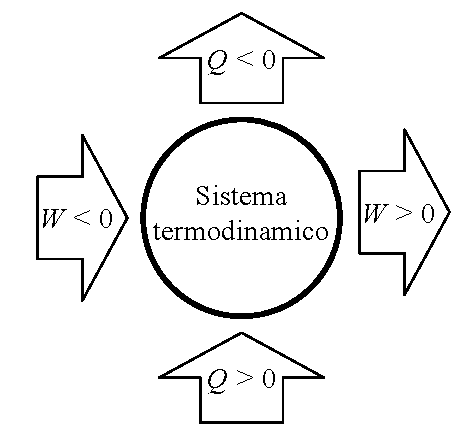
\includegraphics[width = \marginparwidth]{convenzione_segni_flussi_energetici_sistema_termodinamico.pdf}
    \caption{Convenzione sui segni dei flussi energetici in un
    sistema termodinamico, al quale si applica la nostra
    formulazione del primo principio.}\label{fluxi}
\end{marginfigure}

Chiariamo le convenzioni sui segni: supponiamo di avere un sistema
termodinamico che scambia calore con l'ambiente e che può compiere
lavoro. La situazione è mostrata in figura \ref{fluxi}.
Quando il sistema acquista calore dall'ambiente esterno,
il valore di questà quantità sarà positivo. Quando invece il
sistema perde calore, quest'ultimo ha valore negativo. In accordo
con il primo principio, supponendo di ignorare il lavoro, l'energia
interna $U$ del sistema diminuisce quando il calore esce e viceversa
aumenta quando entra nel sistema.
Per il lavoro vale il contrario: quando l'ambiente effettua lavoro
sul sistema, questa quantità di energia in entrata ha valore negativo;
quando invece il sistema effettua lavoro sull'ambiente, esso spende
e perde parte della sua energia interna. Per questo motivo, nel
primo principio, il lavoro viene sottratto alla variazione di energia
totale.

Sottolineamo infine che, nella formulazione \ref{firstprincip},
$\Delta U$ corrisponde alla variazione \textit{totale} di energia
interna del sistema in un dato momento nel quale avviene scambio
di energia. Sono dunque totali anche il calore scambiato
$Q$ e il lavoro effettuato $W$.


\subsection{Modalità di trasmissione del calore}
Come il lavoro può presentarsi in svariate forme, come abbiamo
visto dagli esperimenti di Joule ma già anche dalla meccanica,
anche il calore può essere scambiato in vari modi. Queste modalità
di trasmissione hanno in comune la condizione di \textit{contatto
termico}, ovvero situazioni in cui due corpi sono in grado di
trasmettere calore tra di loro. È importante non confondere il
contatto termico con quello fisico, perché, come vedremo, non
sempre il calore si trasmette solo se due corpi si toccano tra loro.

Altro punto da ricordare è che possiamo distinguere che l'energia
si trasferisce sotto forma di calore perché non si compie lavoro.

\subsubsection{Conduzione}
Nella conduzione, il calore viene scambiato per contatto tra corpi.
Un semplice modello per descrivere questo fenomeno è la finestra di
un edificio.

\subsubsection{Convezione}
Nella convezione, il calore viene scambiato per mezzo di masse calde
in movimento, all'interno di masse più fredde. Questa modalità è
caratteristica dei fluidi, data la necessità del moto. Semplici esempi
di questo fenomeno sono la pentola d'acqua sul fornello acceso e la
lava-lamp.

\subsubsection{Irraggiamento}
L'irraggiamento permette lo scambio di energia per mezzo di onde
elettromagnetiche, quindi senza la necessità di essere in contatto
termico con un corpo. Un esempio è il Sole, che di fatto scalda la
Terra mediante le radiazioni emesse. In realtà non è propriamente
corretto dire che il calore viene trasmesso durante il tragitto tra
i due corpi, ma l'effetto delle onde elettromagnetiche che raggiungono
la destinazione è un aumento di temperatura, che assimiliamo ad uno
scambio di calore.

Una legge degna di nota è la \textit{legge di Stefan-Boltzmann} del
potere emissivo di un corpo

\begin{align}
    \varepsilon = \sigma e T^4
\end{align}

\noindent Questa legge esprime la quantità di energia che un corpo
può emettere per irraggiamento data la sua temperatura. Nella realtà,
un corpo non è in grado di emettere la totalità di questa energia
e per tale motivo è presente un fattore $e$ adimensionale, tale che
$0 < e < 1$. Nel caso ideale $e = 1$ si parla di \textit{corpo nero}.
La quantità

\section{Gas ideali}

\subsection{Leggi dei gas ideali}

\subsubsection*{Prima legge di Gay-Lussac}
\subsubsection*{Seconda legge di Gay-Lussac}
\subsubsection*{Legge di Boyle}

\subsubsection*{Legge di Avogadro}
Esempio di equazione di stato.

\subsection{Lavoro di un gas ideale}
Mostreremo ora parte del principio di funzionamento di un pistone
di un motore a combustione interna. Si tratta di un esempio estremamente
semplificato, perché considereremo gas ideali.
Sappiamo bene che il motore termico di, ad esempio, una motocicletta
genera lavoro per azionare la catena e di conseguenza la ruota posteriore.
Il ``tempo'' nel quale il motore genera lavoro è quello nel quale
avviene lo scoppio, che aumenta violentemente la temperatura e la
pressione dell'aria all'interno del cilindro, spingendo di fatto il
pistone.

\begin{marginfigure}
    \centering
    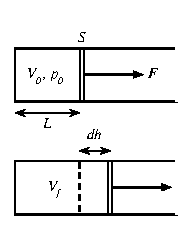
\includegraphics[width = \marginparwidth]{lavoro_gas_ideale.pdf}
    \caption{Lavoro infinitesimo di un gas all'interno di un cilindro.}
    \label{workinggas}
\end{marginfigure}

Si faccia riferimento al motore in figura \ref{workinggas}, costituito
da un cilindro e un pistone libero di muoversi al suo interno. Inizialmente, il pistone,
con sezione di area $S$, si trova ad una distanza $L$ dal fondo del cilindro.
L'aria all'interno ha pressione e volume iniziali $p_0$ e $V_0$. Se l'esterno
del pistone oppone resistenza, il gas del cilindro, avendo una certa pressione,
esercita sulla sezione del pistone una certa forza $\vecsymb{F}$. Immaginiamo
che la resistenza esterna cessi ad un certo istante: il gas, in virtù della forza
esercitata, spingerà il pistone di una certa distanza infinitesima $dh$.
Il gas sta allora compiendo lavoro sul pistone:

\[ dW = \vecsymb{F} \cdot d\vecsymb{s} = Fdh \]

\noindent la forza $F$ non ci è molto utile attualmente. Vogliamo esprimere
tutto sotto forma di variabili termodinamiche e non meccaniche. Notiamo
allora che, dopo lo spostamento $dh$, il gas raggiungerà un certo volume
$V_f$, che è leggermente più voluminoso di $V_0$ di una certa quantità $dV$:

\[ V_f = (L + dh)S = SL + Sdh = V_0 + dV \]

\noindent Tramite semplice algebretta, possiamo dedurre che
$dW = Fdh = \frac{F}{S}Sdh = pdV$. Abbiamo dunque definito
il lavoro infinitesimo di un gas ideale

\begin{align}
    dW = pdV
\end{align}

Stiamo assumendo che, durante l'aumento di $dV$, la pressione
rimanga costante. Se però vogliamo calcolare il lavoro totale
sprigionato durante l'intera corsa del pistone, dobbiamo effettuare
un'integrazione tenendo presente che la pressione varierà durante
tale processo. In generale, data una certa trasformazione termodinamica
$\tau$, il lavoro totale di un gas può essere espresso nella
seguente forma:

\begin{align}
    W_\tau = \int_\tau pdV\label{lavorogas}
\end{align}

\subsubsection*{Il lavoro sul piano $pV$}
Sappiamo bene dalla quinta superiore e da Analisi 1 che gli integrali
sono in qualche modo correlati a interpretazioni geometriche di aree
sottese a grafici. Dalla legge \ref{lavorogas} ottenuta pocanzi si può
notare che il lavoro ``si può vedere'' sul piano $pV$. Dato infatti
il tratto di curva $\tau$ che descrive una trasformazione, il lavoro
$W$ è proprio l'area (con segno) sottesa a $\tau$. In generale,

\begin{itemize}
    \item se il sistema percorre $\tau$ in modo tale da spostarsi nel verso positivo
    dell'asse del volume, il lavoro effettuato dal gas è positivo;

    \item se il sistema si dirige nel verso opposto dell'asse del volume,
    allora il lavoro effettuato è negativo;

    \item se il sistema non si discosta dal proprio volume ($dV = 0$)
    allora il lavoro è nullo.
\end{itemize}

Anticipiamo che esistono trasformazioni particolari, le trasformazioni
\textit{cicliche}, che partendo da una coordinata termodinamica
ritornano sulla medesima dopo la trasformazione, descrivendo un circuito.
In tal caso, il lavoro effettuato dal (o sul) sistema corrisponde
all'area racchiusa nel circuito. La figura mostra intuitivamente le
ragioni di questa proprietà.

\begin{itemize}
    \item Se il sistema percorre il circuito in senso orario, il
    lavoro è positivo.

    \item Se il sistema percorre il circuito in senso antiorario,
    il lavoro è negativo.
\end{itemize}





\subsection{La teoria cinetica dei gas}
È evidente che, nella termodinamica da noi affrontata, il sistema
fisico preferito è quello del gas. Lo abbiamo però sempre trattato
da un punto di vista macroscopico, utilizzando variabili termodinamiche
(pressione, volume e temperatura), senza mai spiegare cosa in realtà
accade nel microscopico, all'interno del gas stesso. È ciò che proveremo
a fare ora, costruendo una teoria che spieghi ciò che osserviamo
dall'esterno. Non abbiamo però altro strumento che quello della meccanica
e per questo motivo i risultati che otterremo in seguito sono
conosciuti sotto il nome di \textit{teoria cinetica dei gas}.

\subsubsection*{Ipotesi e presupposti della teoria}
Sottolineamo che la teoria cinetica, per funzionare, poggia su numerosi
presupposti, molti dei quali sono solo un'approssimazione della realtà.
Tuttavia, vedremo che queste ipotesi condurranno ad una spiegazione
soddisfacente delle nostre osservazioni:

\begin{itemize}
    \item Oggetto della trattazione teorica è un \textit{gas ideale}
    (o perfetto) che si trova all'interno di un contenitore con
    volume $V$. La forma del contenitore non sarà rilevante, ma spesso
    si semplificano i calcoli se esso è un cubo.

    \item Il gas è ideale nel senso che esso è costituito da particelle
    infinitamente piccole rispetto al contenitore e alle distanze che
    le separano. Tali particelle sono inoltre indistinguibili l'una
    dall'altra (eccezion fatta per il loro stato di moto): esse hanno
    in particolare la medesima massa.

    \item Sempre il gas è ideale in quanto a bassa pressione e densità,
    nella misura in cui l'interazione tra le particelle è nulla: non
    avvengono urti e non vi sono interazioni di natura gravitazionale,
    elettrica o di altro genere.

    \item Gli unici urti non trascurabili sono quelli che avvengono
    tra particella e parete del contenitore ed essi sono perfettamente
    elastici, perché tra l'altro la massa delle particelle è infinitamente
    piccola rispetto a quella del contenitore e delle sue pareti. L'urto
    non mette dunque in moto il contenitore.
\end{itemize}

\subsubsection*{La teoria}
Coerentemente con le ipotesi espresse nel paragrafo precedente,
consideriamo ora una singola particella del gas ideale, con massa
$m$. Esso sta per urtare una parete del contenitore cubico, con
lato $L$ e di una certa massa $M$ tale che $M \gg m$. Proiettiamo la situazione su un piano, come in figura
\ref{wall}. La particella potrebbe avere una qualsiasi velocità,
che denoteremo $\vecsymb{v}$. Consideriamo poi solo la componente
orizzontale di tale vettore, ovvero $\vecsymb{v}_x$.

\begin{marginfigure}
    \centering
    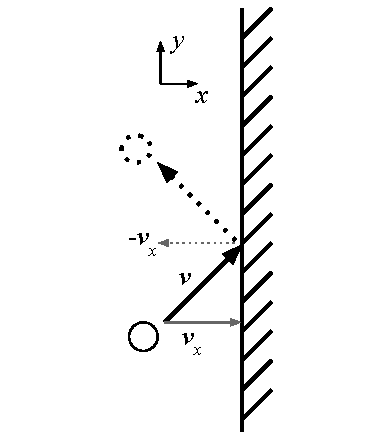
\includegraphics[width = \marginparwidth]{teoria_cinetica_parete.pdf}
    \caption{Urto tra una particella di gas e una delle pareti
    del contenitore.}
    \label{wall}
\end{marginfigure}

Sappiamo dalle equazioni \ref{perfelastico} che l'urto perfettamente
elastico farà rimbalzare la particella in modo tale da rendere
invariato il modulo di $\vecsymb{v}_x$, ma invertendone il verso.
Le quantità di moto finale e iniziale della particella, allora,
corrispondono rispettivamente a $\vecsymb{p}_{x,i} = m\vecsymb{v}_x$
e $\vecsymb{p}_{x,f} = -m\vecsymb{v}_x$. La variazione della quantità
di moto della particella è quindi

\[ \Delta\vecsymb{p}_x = -2mv_x \hat{x} \]

\noindent Utilizziamo il versore $\hat{x}$ per separare i moduli e per trattare
oggetti scalari.

Sappiamo che la variazione $\Delta\vecsymb{p}_x$ può essere interpretata
come un impulso esercitato dalla parete, che quindi esercita una forza
sulla particella. Ma come calcolare questa forza? È necessario trovare
un intervallo temporale entro il quale l'impulso agisce, in modo da
ricavare l'intensità della forza mediante la definizione \ref{impulso}.
Possiamo notare che, per via degli urti perfettamente elastici, la particella
continua a rimbalzare senza che la sua velocità totale $v$ muti.
Proiettando il moto sull'asse $x$, vedremmo il vettore $\vecsymb{v}_x$
invertirsi ciclicamente ad ogni urto con le pareti di destra e sinistra.
La particella impiega allora un tempo

\[ \Delta t = \frac{2L}{v_x} \]

\noindent per lasciare una parete e tornarvici per urtare nuovamente.
Durante questo intervallo di tempo, in media, la forza impulsiva
esercitata da una parete sulla particella ha intensità

\[ F_x = \frac{\Delta p_x}{\Delta t} = 2mv_x \frac{v_x}{2L} = \frac{mv_x^2}{L} \]

\noindent Tramite la definizione di pressione $p = F/S$, (con $S$ la
superficie di una parete, dunque $L^2$) otteniamo la
pressione esercitata dalla singola particella

\[ p_x = \frac{F_x}{L^2} = \frac{mv_x^2}{L^3} = \frac{mv_x^2}{V} \]

\noindent Notare che questo ragionamento vale solo per la componente
$x$, ma lo stesso ragionamento può essere esteso a tutte le altre
componenti. La relazione precedente non è ancora di nostro aiuto,
perché riguarda solo una particolare particella, la cui velocità può
essere differente dalle altre. Calcoliamo dunque la pressione mediante
la forza totale esercitata dalle particelle sull'asse $x$:

\[ F_{\text{tot}, x} = \sum_i F_{x,i} = \sum_i \frac{mv_{x,i}^2}{L} = \frac{m}{L}\sum_i v_{x,i}^2 \]

Supponendo che il gas sia costituito da $N$ particelle, possiamo
effettuare un'approssimazione riducendo le velocità ad una loro media
(essendo al quadrato, sarà una velocità quadratica media).

\[ p_x = \frac{F_{\text{tot},x}}{L^2} = N\frac{m\left\langle v_x^2 \right\rangle}{V} \]

Il ragionamento effettuato per la componente $x$ vale anche per tutte
le altre. Per questo motivo, dato che la pressione è una grandezza
intensiva che idealmente rimane costante in tutto il cubo, possiamo
supporre che $p_x = p_y = p_z = p$. Vogliamo però ottenere un'equazione
che non dipenda da una componente della velocità delle particelle,
ma dalla loro velocità totale. Anche qui supponiamo di ridurre le
velocità di tutte le particelle, che potrebbero differire tra loro,
ad una velocità quadratica media totale. La relazione con le sue
componenti spaziali è ricavabile geometricamente:

\[ \left\langle v^2 \right\rangle  = \left\langle v_x^2 \right\rangle + \left\langle v_y^2 \right\rangle + \left\langle v_z^2 \right\rangle \]

\noindent Le approssimazioni introdotte ci permettono anche di
supporre che tutte e tre le componenti spaziali siano equivalenti
tra loro, ovvero che $\left\langle v_2^2 \right\rangle = \left\langle v_y^2 \right\rangle = \left\langle v_z^2 \right\rangle$.
Usando allora l'equazione della pressione:

\[ p = N\frac{m}{V}\left(\frac13 \left\langle v^2 \right\rangle\right) \]

\noindent Notiamo che compare il prodotto $m\left\langle v^2 \right\rangle$, che
corrisponde al doppio dell'energia cinetica media delle particelle,
$\left\langle E_K \right\rangle$. Otteniamo dunque la seguente relazione:

\[ pV = \frac23 N\left\langle E_K \right\rangle \]

\noindent $\left\langle E_K \right\rangle$ corrisponde ad una singola particella.
Allora possiamo concludere che la somma di tutte le energie cinetiche
medie delle particelle del gas costituiscono l'energia interna del
gas stesso: $E_\text{int} = U = N\left\langle E_K \right\rangle$.
La teoria ci ha dunque permesso dunque di unire le seguenti relazioni:

\[ pV = Nk_BT = \frac23 U \]

In particolare, possiamo notare che

\[ \left\langle E_K \right\rangle = \frac{3}{2}k_B T \]

\noindent che esprime la relazione tra energia cinetica media di una
particella e la temperatura. In un certo senso, la temperatura \textit{è}
l'energia cinetica media delle particelle.

\subsubsection*{Conclusioni}
Il risultato più importante della teoria cinetica è l'unione tra
il mondo macroscopico osservato sperimentalmente e il mondo microscopico
modellato teoricamente. In particolare:
\begin{itemize}
    \item La teoria cinetica offre una spiegazione dell'origine della
    pressione esercitata da un gas in un contenitore. L'origine è proprio
    dovuta alla continua collisione delle particelle con le pareti
    del contenitore.

    \item La teoria cinetica mostra che la temperatura è strettamente
    legata all'energia cinetica media delle particelle. Intuitivamente,
    la temperatura è interpretabile proprio come l'agitazione media
    delle particelle, per l'appunto l'energia del loro movimento.

    \item La teoria cinetica costruisce un modello generalizzabile
    a sistemi di costituenti non necessariamente monoatomico-puntiformi,
    come approfondito nella prossima sezione.
\end{itemize}

\subsubsection*{Gradi di libertà}
Nell'equazione relativa all'energia cinetica media,
il fattore $1/2$ deriva dalla definizione di enrgia cinetica, ma
il numero $3$ invece? Esso dipende dal numero di dimensioni entro
le quali le particelle possono muoversi, ovvero i \textit{gradi di
libertà}. Se compissimo lo studio da capo, costringendo però le particelle
a giacere su un piano, i gradi di libertà sarebbero solo due e il fattore
moltiplicativo
dell'energia cinetica media sarebbe diverso. Ciò è dovuto al fatto
che ogni grado di libertà permette alla particella di muoversi su
un'altra dimensione e quindi di aggiungere un contributo in più alla
propria energia cinetica. In generale, ogni grado di
liberta comporta un contributo energetico di $\frac12k_BT$ e
dunque, per $l$ gradi di libertà, si ottiene

\begin{align}
    \left\langle E_K \right\rangle = \frac{l}{2}k_BT
\end{align}

I gradi di libertà possono crescere all'aumentare della complessità
della particella di gas. Oltre alle tre dimensioni, una molecola
biatomica (quindi non puntiforme come abbiamo sempre supposto finora)
può anche ruotare su due assi\footnote{Due assi sono sufficienti a
coprire tutte le rotazioni nelle tre dimensioni}; i due atomi possono
poi vibrare intorno alla loro ``sede'' nella molecola, dunque anche
questa energia deve essere presa in considerazione. In totale, una
molecola biatomica ideale può avere $l = 6$ gradi di libertà.






\section{Trasformazioni termodinamiche}
Questa sezione è dedicata ad analisi più approfondite sulle trasformazioni
termodinamiche fondamentali, ovvero trasformazioni molto semplici da
trattare mediante gli strumenti di termodinamica finora mostrati. Da
un certo punto di vista, queste trasformazioni rappresentano le modalità
fondamentali con le quali un sistema può muoversi sul piano $pV$. Un
motivo della loro semplicità risiede nel fatto che, in ogni trasformazione,
un qualche parametro termodinamico rimane sempre costante.

Supporremo che queste trasformazioni riguarderanno un gas ideale
contenuto in un cilindro. A seconda del caso di studio, il cilindro
potrà variare il proprio volume interno grazie ad un pistone mobile,
oppure sarà adiabatico. Le trasformazioni saranno inoltre \textit{quasistatiche
reversibili}: ad ogni istante, il sistema è in uno stato di
equilibrio (il passaggio dall'uno all'altro è sufficientemente lento
per raggiungere tale scopo) e inoltre è sempre possibile ripercorrere
la trasformazione, e ogni suo tratto intermedio, in senso inverso.
Le leggi che deriveremo non saranno pertanto applicabili alla lettera
a trasformazioni reali di gas reali, ma costituiranno solo una buona
approssimazione delle osservazioni sperimentali.


\subsection{Isocore}
Queste trasformazioni traggono il loro nome per via del loro volume,
che rimane sempre costante, cioè $dV = 0$. Segue in particolare che
$dW = pdV = 0$, ricordando la definizione di lavoro di un gas ideale.
D'altronde, il volume del gas non cambia e quindi nessuna parte del
suo contenitore viene mossa.

Dal primo principio vale $dU = dQ$. Ciò significa che avviene solo
scambio di calore. Possiamo supporre che il gas, durante la trasformazione,
vari la propria temperatura in relazione al calore scambiato secondo
un certo \textit{calore specifico a volume costante} $c_V$.

\begin{align}
    dQ = nc_VdT
\end{align}

\begin{marginfigure}
    \begin{center}
        \def\xmax{3}
        \def\ymax{2.5}
        \begin{tikzpicture}

        \coordinate (B) at (.5*\xmax,.8*\ymax);
        \coordinate (A) at (.5*\xmax,.2*\ymax);
        
        % LINE
        \draw[very thick,midarr=.55,myred] (A) -- (B);
        \fill (B) circle(0.07) node[right=2,above=2] {$B$};
        \fill (A) circle(0.07) node[right=2] {$A$};
        
        % AXIS
        \draw[->,thick] (0,-0.1*\ymax) -- (0,\ymax) node[anchor=north east] {$p$};
        \draw[->,thick] (-0.1*\xmax,0) -- (\xmax,0) node[anchor=north east] {$V$};
        
        \end{tikzpicture}
    \end{center}
    \caption{Trasformazione isocora sul piano $pV$. Il grafico evidenzia
    molto bene il fatto che il lavoro è nullo, proprio perché il tratto
    $AB$ descrive un segmento verticale che sottende area nulla (volgarmente, non
    ha largezza).}
\end{marginfigure}

\noindent Da cui $dU = nc_VdT$. Come aveva previsto Joule, per questa
particolare trasformazione abbiamo individuato una relazione che lega
energia interna e (variazione di) temperatura di un gas. Ricordando
poi la teoria cinetica, $U = \frac32 nRT$. È facile allora scoprire
che, dati $l$ gradi di libertà per un gas ideale,

\[ c_V = \frac{l}{2}R \]

\noindent per gas monoatomici in tre dimensioni, vale perciò $c_V = \frac32 R$.


\subsection{Isobare}
In queste trasformazioni, è la pressione a rimanere costante.
Calcolarne il lavoro è molto semplice. Si evince infatti che
la definizione si riduce ad una semplice moltiplicazione:
$dW = pdV$, da cui $W = p\Delta V$.

Dalle trasformazioni isocore, abbiamo scoperto un legame tra
variazione di energia interna del gas e variazione di temperatura.
Già per definizione legammo in una funzione queste due quantità.
In particolare, sptabilimmo che $U$ è una funzione di stato, la
cui variazione non dipende dal percorso ma dagli stati iniziale
e finale. Siamo allora legittimati a impiegare la relazione
$dU = nc_VdT$ trovata nelle isocore.

Rimane da trovare il calore scambiato durante una isobara. Anche
qui possiamo inventare una nuova costante, un \textit{calore specifico
a pressione costante} $c_p$, col quale legare calore e intervallo
di temperatura:

\[ dQ = nc_pdT \]

\noindent come per $c_p$, ci piacerebbe conoscere la sua vera forma.
Notiamo che differenziando i membri della legge di Avogadro,
$d[pV] = d[nRT]$, ci ritroveremo con la relazione $pdV = nRdT$,
da cui scopriamo che $dW = nRdT$. Dal primo principio $dU = dQ - dW$,
possiamo allora scoprire che $nc_VdT = nc_pdT - nRdT$, da cui
la \textit{relazione di Mayer}\footnote{Come lo studentato.}

\begin{marginfigure}
    \begin{center}
        % PV diagram - constant P
        \def\xmax{3}
        \def\ymax{2.5}
        \begin{tikzpicture}
        
        % AREA
        \coordinate (A) at (.2*\xmax,.6*\ymax);
        \coordinate (B) at (.8*\xmax,.6*\ymax);
        \coordinate (C) at (.8*\xmax,.2*\ymax);
        \fill[mylightblue] (A) rectangle (C|-0,0) node[midway,blue] {$W$};
        
        % LINE
        \draw[very thick,midarr=.55,myred] (A) -- (B);
        %\draw[very thick,midarr=.55,blue] (B) -- (C);
        \fill (A) circle(0.07) node[right=2,above=2] {$A$};
        \fill (B) circle(0.07) node[right=2,above=2] {$B$};
        %\fill (C) circle(0.07) node[right=2] {$P_2$, $V_2$};
        
        % AXIS
        \draw[->,thick] (0,-0.1*\ymax) -- (0,\ymax) node[anchor=north east] {$p$};
        \draw[->,thick] (-0.1*\xmax,0) -- (\xmax,0) node[anchor=north east] {$V$};
        
        \end{tikzpicture}
    \end{center}
    \caption{Trasformazione isobara sul diagramma $pV$. La
    pressione in $A$ è uguale a quella in $B$. Notare come
    il lavoro $W$ può essere facilmente calcolato: corrisponde
    proprio all'area del rettangolo azzurro, che ha per base
    $\Delta V = V_B - V_A$ e altezza $p_A = p_B$.}
\end{marginfigure}

\begin{tcolorbox}[colback = red!30, colframe = red!30!black, title = {Relazione di Mayer}]
\begin{align}
    c_p - c_V = R
\end{align}
\end{tcolorbox}

\noindent La relazione ci permette di esprimere $c_p$ per gas
monoatomici in tre dimensioni: $c_p = c_V + R = \frac52 R$.
Osserviamo infine che

\begin{align}
    c_p > c_V
\end{align}

\noindent È facile spiegare intuitivamente
il perché di questa disuguaglianza: a parità di calore fornito ad
una certa quantità di gas, è maggiore la differenza di temperatura
registrata dal gas a volume costante, perché esso non disperde il
calore fornito in lavoro, come invece accade per il gas a pressione
costante (in quest'ultimo, possiamo immaginare che il contenitore
possieda un pistone mobile. Fornendo calore al gas, la pressione
può rimanere costante a costo di muovere il pistone).

Per finire, tenete bene a mente questa definizione:

\begin{align}
    \gamma = \frac{c_p}{c_V}\label{gamgam}
\end{align}

\noindent il motivo: ci tornerà utile in una delle prossime trasformazioni.
Spendiamo qualche ultima parola sul termine $\gamma$:
ricordando che al crescere della complessità delle molecole del
gas crescono i loro gradi di libertà $l$, concludiamo che

\[ \lim_{l \to +\infty} \gamma(l) = 1 \]

\noindent Questo risultato ci suggerisce che all'aumentare della
complessità della molecola, i calori specifici del gas a pressione
e volume costante sono pressoché uguali.

\subsection{Isoterme}
Come si evince dal nome, queste trasformazioni avvengono a temperatura
costante. Come già visto con la legge di Boyle, per il gas ideale
vale $pV = \text{ cost.} = nRT$. Per questo motivo, $dT = 0$, da cui
$dU = nc_VdT = 0$ (come prima, esprimiamo la variazione di energia
interna sfruttando il calore specifico a volume costante). Sempre in
accordo con le precedenti osservazioni, se la temperatura non varia
allora anche l'energia interna del gas rimane costante. Dal primo
principio segue allora

\[ dQ = dW \]

\noindent da cui $dQ = dW = pdV = nRT\frac{dV}{V}$ per definizione di lavoro
di un gas ideale. Segue dunque che:

\begin{align}
    Q = W = \int_{V_i}^{V_f}nRT\frac{dV}{V} = nRT\ln\left(\frac{V_f}{V_i}\right)
\end{align}

\begin{marginfigure}
    \begin{center}
        % PV diagram - isotherm
        \begin{tikzpicture}
            \def\N{40} % number of plot samples
            \def\xmax{3}
            \def\ymax{2.5}
            \def\isotherm{(A) to[out=-60,in=170] (B)}
            \def\T{1.2}
            \def\xa{.2*\xmax}
            \def\xb{.8*\xmax}
            \def\ya{{\T/(\xa)}}
            \def\yb{{\T/(\xb)}}
            
            % AREA
            \coordinate (A) at (\xa,\ya);
            \coordinate (B) at (\xb,\yb);
            \fill[mylightblue,samples=\N,domain=\xa:\xb]
            plot(\x,{\T/\x}) -- (B|-0,0) -- (A|-0,0) node[midway,left=4,above=5,blue] {$W$} -- cycle;
            
            % LINE
            \draw[myred,very thick,midarr=.58,samples=\N,domain={\xa}:{\xb}]
            plot(\x,{\T/\x});
            \fill (A) circle(0.07) node[right=5,above=2] {$A$};
            \fill (B) circle(0.07) node[right=2] {$B$};
            
            % AXIS
            \draw[->,thick] (0,-0.1*\ymax) -- (0,\ymax) node[anchor=north east] {$p$};
            \draw[->,thick] (-0.1*\xmax,0) -- (\xmax,0) node[anchor=north east] {$V$};
            
        \end{tikzpicture}
    \end{center}
    \caption{Trasformazione isoterma sul piano $pV$. Il
    grafico corrisponde ad un tratto di ramo di iperbole
    equilatera. Tutti i punti sul ramo rappresentano stati
    ad una certa temperatura $T$.}
\end{marginfigure}

\subsubsection*{Considerazioni}
Si noti che, per ottenere il calore scambiato, non ha
senso inventarsi, come per le altre trasformazioni, un calore specifico
a temperatura costante $c_T$, perché la sua eventuale definizione
$dQ = nc_TdT$ non funzionerebbe: $dT = 0$, da cui concluderemmo erroneamente che
$dQ = 0$! In una trasformazione isoterma è possibile
mantenere una temperatura costante del gas a patto di convertire
calore in lavoro o viceversa. Se ad esempio si riceve lavoro dall'ambiente esterno,
esso viene contemporaneamente dissipato in calore in uscita, altrimenti
l'energia interna del gas (quindi la sua temperatura) aumenterebbe.
Per questo motivo, possiamo determinare la quanità di calore in una
isoterma a partire dal lavoro.


\subsection{Adiabatiche}
Se nelle trasformazioni isocore non si osserva lavoro in azione, nelle
adiabatiche non si registra invece scambio di calore: $dQ = 0$, da cui,
sempre per il primo principio, $dU = -dW$. Anche qui possiamo utilizzare
la scorciatoia di $c_V$ per concludere che $dU = nc_VdT$.
Dalla relazione $dU = -dW$ possiamo trarre conclusioni interessanti.
Possiamo infatta esprimerla come $nc_VdT = -pdV$. Proseguendo,

\begin{align*}
    nc_VdT &= -pdV\\
    \not n c_VdT &= -\not n RT\frac{dV}{V}\\
    \frac{dT}{T} &= -\frac{R}{c_V}\frac{dV}{V}
\end{align*}

\begin{marginfigure}
    \begin{center}
        \begin{tikzpicture}
            \def\N{40} % number of plot samples
            \def\Th{2.5}
            \def\Tc{.8}
            \def\Ch{2.4}
            \def\gam{2}
            \def\A{ (\Th/\Ch)^(1/(1-\gam)) }
            \def\B{ (\Tc/\Ch)^(1/(1-\gam)) }
            \def\isotherm#1#2{{ #2/(#1) }}
            \def\adiabatic#1#2{{ #2/(#1)^(\gam) }}
            \def\xmax{3.5}
            \def\ymax{2.5}

            \coordinate (A) at ({\A},{\isotherm{\A}{\Th}});
            \coordinate (B) at ({\B},{\isotherm{\B}{\Tc}});
            
            % WORK
            \fill[mylightblue,domain={\A:\B},samples=\N]
              plot (\x,\adiabatic{\x}{\Ch}) |- (A|-0,0) -- cycle;
            
            \node[blue] at ($(B-|A)!.25!(B)+(0,.14)$) {$W$};

            % ISOTHERMS
            \draw[mydarkblue,thick,
                  domain={\isotherm{1.1*\ymax}{\Th}}:{1*\xmax},samples=\N,dashed]
              plot (\x,\isotherm{\x}{\Th});

            % ADIABATIC
            \draw[myred,thick,midarr=.48,
                  domain={\A:\B},samples=\N]
              plot (\x,\adiabatic{\x}{\Ch});
            
            % POINTS
            \fill[black] (A) circle(0.05) node[right = 2, above = 2] {$A$};
            \fill[black] (B) circle(0.05) node[right = 2, above = 2] {$B$};
            
            % AXIS
            \draw[->,thick] (0,-0.1*\ymax) -- (0,\ymax+0.1)
              node[anchor=north east,inner sep=4,scale=1] {$p$};
            \draw[->,thick] (-0.1*\xmax,0) -- (\xmax+0.1,0)
              node[anchor=north east,inner sep=4,scale=1] {$V$};
            
          \end{tikzpicture}
    \end{center}
    \caption{Trasformazione adiabatica sul piano $pV$. La curva
    adiabatica appare più ripida dell'isoterma, rappresentata
    dalla curva tratteggiata. Più $\gamma$ cresce, più la pendenza
    dell'adiabatica si
    fa forte. Ricordiamo però che $\gamma$ può al più avvicinarsi
    a 1.}
\end{marginfigure}

\noindent notiamo che l'algebretta e la relazione di Mayer
ci portano a scoprire che $R/c_V = (c_p - c_V)/c_V = \gamma - 1$
(ricordate la \ref{gamgam}?). Possiamo allora scrivere

\begin{align*}
    \frac{dT}{T} &= -(\gamma - 1)\frac{dV}{V}\\
    \int_{i}^{f}\frac{dT}{T} &= \int_{i}^{f}-(\gamma - 1)\frac{dV}{V}\\
    \ln\left(\frac{T_f}{T_i}\right) &= -(\gamma - 1)\ln\left(\frac{V_f}{V_i}\right)\\
    T_fV_f^{\gamma - 1} &= T_iV_i^{\gamma - 1}
\end{align*}

\noindent vedere un prodotto che rimane sempre costante solletica le
meningi dei fisici. Dall'ultima equazione si conclude che

\begin{align}
    TV^{\gamma - 1} = \text{ cost.}\label{lativuu}
\end{align}

\noindent Lasciamo al lettore l'esercizio di ricavare le altre
espressioni di questa relazione, ovvero utilizzando le altre
variabili termodinamiche\footnote{Scherzone, forniamo qui
la legge espressa in pressione-volume: $pV^\gamma = \text{cost}$
(avete ottenuto la stessa equazione? Sì? Scossa? [\texttt{attesa
pressante}] Va beneee). Lo facciamo perché possiamo spiegare
matematicamente l'andamento dell'adiabatica sul piano $pV$.}.

\subsection[Sunto, trasformazioni composte e cicliche, reversibilità]{Riassunto, trasformazioni composte e cicliche, reversibilità nelle trasformazioni}
Le sezioni precedenti introducono i mattoncini fondamentali per
trattare molti problemi termodinamici semplici. Esistono altre
trasformazioni, più o meno complesse, che però ricorrono a
calcoli più lunghi oppure a strumenti matematici al di fuori
della nostra portata.
Di seguito riportiamo alcune considerazioni sulle trasformazioni
appena introdotte.

\subsubsection*{Tabella riassuntiva}
Sappiamo bene che le tabelle riassuntive piacciono a tutti quando
si parla di leggi da memorizzare.

\begin{center}
    \begin{tabular}{c | c | c | c | c}
        & Isocora & Isobara & Isoterma & Adiabatica\\
        & $\Delta V = 0$ & $\Delta p = 0$ & $\Delta T = 0$ & $Q = 0$\\
        \hline
        \hline
        $\Delta U$ & $nc_V\Delta T$ & $nc_V\Delta T$ & 0 & $nc_V\Delta T$\\
        \hline
        $Q$ & $nc_V\Delta T$ & $nc_p\Delta T$ & $nRT\ln(V_f/V_i)$ & 0\\
        \hline
        $W$ & 0 & $nR\Delta T = p\Delta V$ & $nRT\ln(V_f/V_i)$ & $-nc_V\Delta T$
    \end{tabular}
    \captionof{table}{Leggi utili delle trasformazioni fondamentali.}
    \label{tabellazza_riassuntazza}
\end{center}

\subsubsection*{Trasformazioni composte e cicliche}
Combinando insieme le trasformazioni semplici viste fino ad ora, è possibile
comporre trasformazioni più complesse. Ad esempio, un gas in certe
condizioni di pressione e volume può passare ad un altro stato mediante
una adiabatica, seguita da una isoterma e infine da una isobara. %FIGURA!!!
Tra tutte queste trasformazioni ``composte'', quelle più interessanti
sono forse le trasformazioni cicliche (o cicli termodinamici), nelle
quali, data una coordinata termodinamica, il sistema ritorna nello stesso
punto dopo aver compiuto alcune trasformazioni. Seguendo i nostri presupposti,
possiamo concludere che la variazione di energia interna dei sistemi che
subiscono trasformazioni cicliche non varia tra giri consecutivi:

\[ \Delta U_\tau = 0 \quad \forall \tau \text{ ciclica} \]

\noindent in quanto quest'ultima dipende unicamente dallo stato. Se
lo stato iniziale e finale coincidono, non vi sono variazioni di energia
interna.
Le trasformazioni cicliche costituiscono il principio di funzionamento delle macchine.

Mostriamo un esempio di trasformazione ciclica, con calcoli
annessi:


\subsubsection*{Reversibilità e irreversibilità}
Abbiamo affermato che le leggi che descrivono le trasformazioni fondamentali
valgono solamente nel caso ideale di trasformazioni reversibili.

\begin{tcolorbox}[colback = yellow!30, colframe = yellow!30!black, title = {Trasformazioni reversibili}]
    Un processo si dice reversibile se esso, in qualche modo, è
    invertibile così da riportare l'universo allo stato
    precedente.
\end{tcolorbox}

\noindent L'ipotesi di reversibilità ci consente di utilizzare senza
pensieri le leggi della tabella \ref{tabellazza_riassuntazza}. Inoltre,
il verso di percorrenza delle trasformazioni reversibili può essere
tranquillamente invertito, a patto di rispettare le convenzioni sui
segni delle quantità di energia che vengono scambiate.

È estremamente importante leggere la definizione senza perdere alcun
dettaglio: \emph{l'universo} (sistema e ambiente esterno insieme) deve poter
essere riportato indietro, prima che la trasformazione avvenisse.
Per spiegare meglio il concetto, prendiamo come esempio un cubetto di ghiaccio e una tazza di
té\footnote{Té o the? Boh, mai capito quale dei due sia giusto.} bollente.
Inavvertitamente, facciamo cadere il ghiaccio nella tazza e,
con indifferente stupore, osservando il cubetto gelido nella bevanda
incandescente, vedremmo il primo dissolversi lentamente nell'intruglio.
Il latte è ormai stato versato, ma vorremmo ritornare indietro e
recuperare quel disgraziato cubetto. Recuperiamo allora un po' di acqua
del té e la ricongeliamo nel freezer. Ed ecco che il nostro cubetto
è di nuovo nelle nostre mani.

Ma siamo sicuri di aver riportato proprio \emph{tutto l'universo}
allo stato iniziale? Non solo il ghiaccio, ma anche il té, la tazza,
l'intero ambiente nel quale tutto ciò è avvenuto? Purtroppo, il prossimo
capitolo mostra che queste domande trovano risposta negativa. Il motivo
non lo possiamo ancora comprendere; possiamo solo dire che il processo
di scioglimento del ghiaccio è stato irreversibile e in verità lo sono
tutti quelli che vediamo nella realtà: oggetti che bruciano e si consumano,
gas che si espandono, stelle che muoiono. Tutto questo non può essere
riportato come era esattamente all'inizio, ambiente esterno compreso.
Si tratta di una legge di natura. Perché allora siamo riusciti a riottenere
il cubetto di ghiaccio dell'esempio precedente? In realtà, questo è possibile
a spese di qualcos'altro: il congelatore che consuma corrente elettrica,
prodotta chissà dove mediante trasformazioni irreversibili. Anticipiamo
peraltro che queste spese prese in carico dall'ambiente esterno sono
maggiori nel caso in cui si desidera tornare indietro.